% To familiarize yourself with this template, the body contains
% some examples of its use.  Look them over.  Then you can
% run LaTeX on this file.  After you have LaTeXed this file then
% you can look over the result either by printing it out with
% dvips or using xdvi.
%

\documentclass[twoside,english]{article}
\setlength{\oddsidemargin}{0.25 in}
\setlength{\evensidemargin}{-0.25 in}
\setlength{\topmargin}{-0.6 in}
\setlength{\textwidth}{6.5 in}
\setlength{\textheight}{8.5 in}
\setlength{\headsep}{0.75 in}
\setlength{\parindent}{0 in}
\setlength{\parskip}{0.1 in}

%
% ADD PACKAGES here:
%

\usepackage{amsmath,amsfonts,graphicx,algorithm,caption}
\usepackage[noend]{algpseudocode}
\usepackage{hyperref}
\usepackage{natbib}
\usepackage[document]{ragged2e}
\usepackage{graphicx} %package to manage images
\usepackage{amsmath}
\usepackage{mathtools}
%
% The following commands set up the lecnum (lecture number)
% counter and make various numbering schemes work relative
% to the lecture number.
%
\newcounter{lecnum}
\renewcommand{\thepage}{\arabic{page}}
\renewcommand{\thesection}{\arabic{section}}
\renewcommand{\theequation}{\arabic{equation}}
\renewcommand{\thefigure}{\arabic{figure}}
\renewcommand{\thetable}{\arabic{table}}
\makeatletter
\def\BState{\State\hskip-\ALG@thistlm}
\makeatother
%
% The following macro is used to generate the header.
%
\newcommand{\lecture}[4]{
   \pagestyle{myheadings}
   \thispagestyle{plain}
   \newpage
   %\setcounter{lecnum}{#1}
   \setcounter{page}{1}
   \noindent
   \begin{center}
   \framebox{
      \vbox{\vspace{2mm}
    \hbox to 6.28in { {\bf IE506: Machine Learning - Principles and Techniques
		\hfill Jan-May 2025} }
       \vspace{4mm}
       \hbox to 6.28in { {\Large \hfill Final Review Report : #1  \hfill} }
       \vspace{2mm}
       \vspace{2mm}
       \hbox to 6.28in { {\it Team Name: #2 \hfill Team Members: #3} }
       %\vspace{2mm}}
       %\hbox to 6.28in { {\it Due Date: 01-August-2018} }
      \vspace{2mm}}
   }
   \end{center}
%   \markboth{Assignment #1: #2}{Assignment #1: #2}

   %{\bf Note}: {\it LaTeX template courtesy of UC Berkeley EECS dept.}

   %{\bf Disclaimer}: {\it These notes have not been subjected to the
   %usual scrutiny reserved for formal publications.  They may be distributed
   %outside this class only with the permission of the Instructor.}
   \vspace*{4mm}
}
%
% Convention for citations is authors' initials followed by the year.
% For example, to cite a paper by Leighton and Maggs you would type
% \cite{LM89}, and to cite a paper by Strassen you would type \cite{S69}.
% (To avoid bibliography problems, for now we redefine the \cite command.)
% Also commands that create a suitable format for the reference list.
\renewcommand{\cite}[1]{[#1]}
\def\beginrefs{\begin{list}%
        {[\arabic{equation}]}{\usecounter{equation}
         \setlength{\leftmargin}{2.0truecm}\setlength{\labelsep}{0.4truecm}%
         \setlength{\labelwidth}{1.6truecm}}}
\def\endrefs{\end{list}}
\def\bibentry#1{\item[\hbox{[#1]}]}

%Use this command for a figure; it puts a figure in wherever you want it.
%usage: \fig{NUMBER}{SPACE-IN-INCHES}{CAPTION}
\newcommand{\fig}[3]{
			\vspace{#2}
			\begin{center}
			Figure #1:~#3
			\end{center}
	}
% Use these for theorems, lemmas, proofs, etc.
\newtheorem{theorem}{Theorem}[lecnum]
\newtheorem{lemma}[theorem]{Lemma}
\newtheorem{proposition}[theorem]{Proposition}
\newtheorem{claim}[theorem]{Claim}
\newtheorem{corollary}[theorem]{Corollary}
\newtheorem{definition}[theorem]{Definition}
\newenvironment{proof}{{\bf Proof:}}{\hfill\rule{2mm}{2mm}}

% **** IF YOU WANT TO DEFINE ADDITIONAL MACROS FOR YOURSELF, PUT THEM HERE:
\newcommand{\R}{\mathbb{R}}

\begin{document}
%FILL IN THE RIGHT INFO.
%\lecture{**LECTURE-NUMBER**}{**DATE**}{**LECTURER**}{**SCRIBE**}
\lecture{Creating Graphics Programs from Images}{Your team's name}{Roll numbers of team members}
%\footnotetext{These notes are partially based on those of Nigel Mansell.}

% **** YOUR NOTES GO HERE:

% Some general latex examples and examples making use of the
% macros follow.  
%**** IN GENERAL, BE BRIEF. LONG SCRIBE NOTES, NO MATTER HOW WELL WRITTEN,
%**** ARE NEVER READ BY ANYBODY.

%\begin{abstract}
%	This project report contains the details on our project which aims to infer graphics software programs from hand-drawn images. We describe the deep learning tools involved in our project. In particular, we explain about the deep neural network architectures, the loss functions and activation functions used and the training algorithm used. We have tried a new deep learning architecture and superior results are presented using the proposed architecture.  
%\end{abstract}

\section{Problem Statement}

Provide a short introduction about the project with proper motivation and applications. Give a broad overview of the problem statement that has been tackled in the project.

\section{Work Done Before Stage-1 Review} \label{sec:stage1}
This section can be populated from the proper details about the work done before the stage-1 review. You are expected to include all essential details that explain the work done till the stage-1 review.

An example for the description and citation can be seen as follows.

The neural network to infer spec $S$ from an input image $I$ uses ideas from Neurally guided procedural models \citep{paper2} and attend-infer-repeat \citep{paper3} models. The network is trained on sampled specs $S$ and target images $I$ from randomly generated scenes. The network is trained by maximizing the parametrized likelihood $P_\theta(S|I)$ of inferring a spec $S$ given an image $I$, with the parameters $\theta$ being the parameters associated with the neural network. The network structure is illustrated in Figure \ref{specgenimg}. For further robustness to correct the network errors, the network outputs are further processed by a sequential Monte Carlo sampling scheme \citep{book1}.    
  
\begin{figure}[!h]
	\centering
	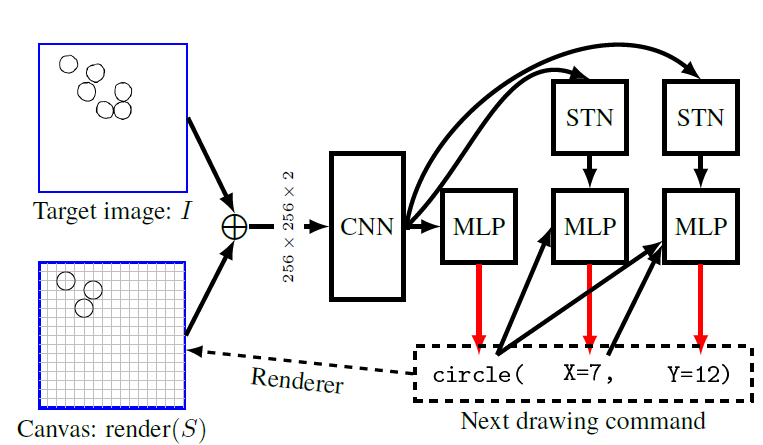
\includegraphics[scale=0.8]{specgen}
	\caption{Neural architecture to infer specs from images.}\label{specgenimg}
\end{figure}



\section{Comments/Inputs given during the Stage-1 Review} \label{sec:stage1_comments}

Give details on the comments that were provided during the stage-1 review.

\subsection{Addressing Comments after Stage-1 Review}
Brief summary on what measures have been taken by team to address the comments. 

\section{Experiments and Replications of Algorithms in Paper} 

In this section discuss all experimental settings, dataset details and experimental results are discussed with a proper summary. Include quantitative results in the form of tables and plots where necessary. Also include qualitative results wherever applicable.
\section{Novel Settings and Experiments} \label{sec:novel}

Explain all details  on the data sets used for the project. Description of data size and attributes, nature and type of data (image/audio/text/video etc.), data pre-processing techniques used should be illustrated. Other relevant details on data procurement (the website from where the data is obtained), and how the data is to be used in experiments should be described. 

\section{Conclusion} \label{sec:conclusion}

Conclude by giving a summary of your project, summarizing the problem, the methods used, and the significance of results obtained. Give some indications of future work to be done. 

\section{Contributions} \label{sec:contribution}
Insert bullet points on individual contributions of the teammates towards the project.



\bibliographystyle{plain}
\bibliography{demo} % Because the file name is demo.bib


\end{document}

